\chapter{Numerical Methods Implementation}

\section{Overall Numerical Strategy, Computational Grid, and Data Layout}
\label{sec:numimpl_overview_grid}

This chapter describes how the Gray--Scott reaction--diffusion model is solved numerically and how the final MATLAB implementation realizes the method in practice. The goal is not only to state the discrete equations, but also to explain how the final code organizes the solver, stores the state variables, applies the diffusion operator, and keeps the different solver variants consistent with each other.
The final program is implemented in MATLAB R2025b and follows a deliberately modular design. The physical model is represented by two coupled scalar fields, $u(x,y,t)$ and $v(x,y,t)$, on a two-dimensional rectangular domain. In the code, the complete simulation pipeline is organized in the following sequence:
\begin{quote}
\small\ttfamily
defaultParams $\rightarrow$ finalizeParams $\rightarrow$ buildGrid $\rightarrow$ makeOperator $\rightarrow$\\ GrayScottModel $\rightarrow$ eulerStep
\end{quote}
This separation is important for both correctness and maintainability. Parameter definition, grid generation, operator construction, time stepping, plotting, and file export are not mixed in one monolithic script. Instead, each step has a well-defined responsibility, which makes the solver easier to verify, extend, and defend.

From the numerical point of view, the solver uses a method-of-lines style discretization. Space is discretized first on a uniform Cartesian grid, which transforms the partial differential equations into a coupled system of ordinary differential equations in time. These semi-discrete equations are then advanced by an explicit Euler method. Within each time step, the code computes the diffusion contribution, the nonlinear reaction contribution, optional source terms used for manufactured-solution tests, and finally the boundary-condition overwrite where required. This design keeps the mathematical structure of the Gray--Scott system visible in the implementation and makes the individual numerical ingredients easy to inspect separately.

The computational domain is defined as
\[
\Omega = [0,L_x)\times[0,L_y),
\]
with $N_x$ grid points in the $x$-direction and $N_y$ grid points in the $y$-direction. The corresponding uniform grid spacings are
\begin{equation}
h_x = \frac{L_x}{N_x},
\qquad
h_y = \frac{L_y}{N_y}.
\label{eq:grid_spacing_numimpl}
\end{equation}
The grid points are therefore
\[
x_i = i h_x,\qquad i=0,1,\dots,N_x-1,
\]
\[
y_j = j h_y,\qquad j=0,1,\dots,N_y-1.
\]
The right endpoint is excluded in both directions. This is a deliberate and important implementation choice. For periodic boundary conditions, the points at $x=0$ and $x=L_x$ represent the same physical location, and similarly for $y=0$ and $y=L_y$. Including both endpoints would therefore duplicate one grid line and would make the periodic indexing inconsistent. The function \texttt{buildGrid.m} follows exactly this convention and constructs the grid on $[0,L_x)\times[0,L_y)$ rather than on $[0,L_x]\times[0,L_y]$.

In the final code, periodic boundaries are the default configuration, but the user may also select Dirichlet or Neumann conditions independently on each side of the domain. This flexibility is handled through the boundary-condition structure stored in \texttt{p.BC}. The important design choice is that the grid itself remains the same for all boundary types. In other words, the discretization does not change from one grid layout to another when the user switches boundary conditions. Instead, the solver keeps one consistent grid representation and applies the selected boundary treatment during the update process. This avoids unnecessary code duplication and keeps the main numerical kernel uniform across different simulation setups.

The state variables are stored in two complementary forms. For numerical operations that naturally act on the two-dimensional field, the concentrations are represented as arrays
\[
U \in \mathbb{R}^{N_y \times N_x},
\qquad
V \in \mathbb{R}^{N_y \times N_x}.
\]
This is convenient for initialization, visualization, stencil-based diffusion, and explicit boundary updates. However, for matrix-based operator application and for a clean algebraic formulation, the same fields are also stored in vectorized form:
\[
u = U(:),
\qquad
v = V(:).
\]
The final solver therefore uses a deliberate dual representation: two-dimensional arrays for field-based logic and one-dimensional vectors for operator-based logic. This is one of the key implementation decisions of the project because it allows the sparse matrix, dense matrix, and matrix-free stencil realizations to share the same mathematical interpretation.

The vectorization follows MATLAB's column-major memory layout. If $U(j,i)$ denotes the field value at grid index $(i,j)$, then the corresponding vector index is
\begin{equation}
k = j + (i-1)N_y,
\qquad
i=1,\dots,N_x,\quad j=1,\dots,N_y.
\label{eq:column_major_mapping_numimpl}
\end{equation}
This means that the $y$-index varies fastest in memory, while the $x$-index advances in blocks of size $N_y$. The choice is not arbitrary; it is exactly the storage convention used internally by MATLAB when a matrix is reshaped or flattened. As a result, the operations
\[
u = U(:), \qquad U = \texttt{reshape}(u,N_y,N_x)
\]
are fully consistent and do not require any manual permutation of indices. This consistency is essential for the correctness of the Kronecker-product Laplacian, because the matrix assembly must follow the same indexing convention as the state vectors used in time stepping.

The same storage convention also explains an important aspect of the implementation architecture. The sparse and dense operator backends apply the discrete Laplacian by matrix--vector multiplication, whereas the stencil backend reshapes the vector back into a two-dimensional field, evaluates neighbor contributions directly in array form, and then re-vectorizes the result. Since all three backends are tied to the same column-major mapping, they represent the same discrete spatial operator even though their internal realization differs. This common data layout is one of the reasons why equivalence tests between the matrix and stencil solvers can be performed in a clean and reliable way.

Another important practical aspect is the initialization of the state. The function \texttt{initialCondition.m} creates two $N_y \times N_x$ arrays, initially with $U=1$ and $V=0$, and then inserts a centered square perturbation region with modified concentrations. Small random perturbations can be added as well. Reproducibility is ensured through a user-defined random seed stored in the parameter structure and activated when the \texttt{GrayScottModel} object initializes or resets the state. This means that two runs with the same parameters and the same seed reproduce the same initial fields, which is essential for fair solver comparison, GUI consistency tests, and benchmark reproducibility.

The final code also caches the initial boundary values when a Dirichlet boundary is selected in \texttt{initial} mode. This is an implementation detail with clear numerical motivation. If a boundary is supposed to remain equal to the initial state, those values must be preserved explicitly rather than reconstructed later. The constructor of \texttt{GrayScottModel} therefore stores a boundary cache after initialization, so that subsequent time steps can re-impose the correct boundary values consistently. This is a good example of how the final software design supports the intended mathematical meaning of the boundary conditions.

At the highest level, the simulation state is encapsulated in the class \texttt{GrayScottModel}. This class stores the parameter structure, the grid, the chosen diffusion operator, the current state vectors, and the current simulation time and step counter. The actual one-step update is delegated to \texttt{eulerStep.m}, which receives the current vectors and returns the updated state plus diagnostic information. This separation is useful because it keeps the state management logic inside the model object while the numerical update rule remains transparent as a standalone function. The solver is not just a script that repeatedly modifies variables, but a structured numerical program with a clear distinction between model state, operator construction, and one-step evolution.

In summary, the final implementation is built around three core ideas: a uniform Cartesian grid on $[0,L_x)\times[0,L_y)$, a column-major data layout consistent with MATLAB's native memory model, and a modular solver architecture that cleanly separates parameter handling, operator realization, and time stepping. These choices are not merely programming preferences; they directly support the numerical method, make the different solver variants comparable, and provide a robust foundation for the more detailed discretization and implementation discussions that follow in the next sections.

\section{Spatial Discretization and the Discrete Laplacian}
\label{sec:numimpl_spatial_laplacian}

After defining the computational grid and the data layout, the next step is the spatial discretization of the diffusion term. In the Gray--Scott system, diffusion acts through the Laplacian operator on both concentration fields,
\[
D_u \nabla^2 u,
\qquad
D_v \nabla^2 v.
\]
The final solver approximates this operator on the uniform Cartesian grid introduced in the previous section by the standard second-order central finite-difference formula. This leads to the classical five-point stencil in two space dimensions.

Let $U(j,i)$ denote the grid value of a scalar field at the point $(x_i,y_j)$, with
\[
i=0,1,\dots,N_x-1,
\qquad
j=0,1,\dots,N_y-1.
\]
For a uniform grid, the second derivative in the $x$-direction is approximated by
\begin{equation}
\frac{\partial^2 u}{\partial x^2}(x_i,y_j)
\;\approx\;
\frac{U(j,i+1)-2U(j,i)+U(j,i-1)}{h_x^2},
\label{eq:uxx_central_numimpl}
\end{equation}
and similarly in the $y$-direction,
\begin{equation}
\frac{\partial^2 u}{\partial y^2}(x_i,y_j)
\;\approx\;
\frac{U(j+1,i)-2U(j,i)+U(j-1,i)}{h_y^2}.
\label{eq:uyy_central_numimpl}
\end{equation}
Adding these two contributions gives the discrete Laplacian
\begin{equation}
(\Delta_h U)(j,i)
=
\frac{U(j,i+1)-2U(j,i)+U(j,i-1)}{h_x^2}
+
\frac{U(j+1,i)-2U(j,i)+U(j-1,i)}{h_y^2}.
\label{eq:laplacian_5point_numimpl}
\end{equation}
This expression corresponds to the standard five-point finite-difference stencil on a two-dimensional Cartesian grid. The local coupling pattern of this operator is shown in Figure~\ref{fig:five_point_stencil}. On a uniform grid, the approximation is second-order accurate in space, provided that the continuous solution is sufficiently smooth. Since the final code also supports rectangular domains with different mesh spacings in the two coordinate directions, the implementation retains the factors $1/h_x^2$ and $1/h_y^2$ separately rather than assuming $h_x=h_y$.

\begin{figure}[H]
  \centering
  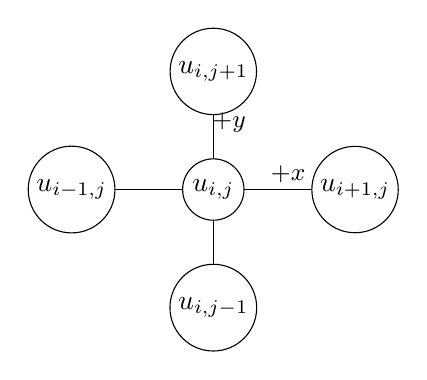
\begin{tikzpicture}[scale=1.0, line cap=round, line join=round]
    % Nodes
    \node[circle, draw, inner sep=2pt] (C) at (0,0) {$u_{i,j}$};
    \node[circle, draw, inner sep=2pt] (N) at (0,1.5) {$u_{i,j+1}$};
    \node[circle, draw, inner sep=2pt] (S) at (0,-1.5) {$u_{i,j-1}$};
    \node[circle, draw, inner sep=2pt] (E) at (1.8,0) {$u_{i+1,j}$};
    \node[circle, draw, inner sep=2pt] (W) at (-1.8,0) {$u_{i-1,j}$};

    % Connections
    \draw[-] (C) -- (N);
    \draw[-] (C) -- (S);
    \draw[-] (C) -- (E);
    \draw[-] (C) -- (W);

    % Direction labels
    \node at (0.95, 0.2) {\small $+x$};
    \node at (0.2, 0.85) {\small $+y$};
  \end{tikzpicture}
  \caption{Five-point finite-difference stencil used for the discrete Laplacian on the two-dimensional Cartesian grid.}
  \label{fig:five_point_stencil}
\end{figure}

The physical interpretation of \eqref{eq:laplacian_5point_numimpl} is straightforward. The value at each interior node is compared with its four nearest neighbors: east, west, north, and south. If the center value is larger than the neighborhood average, diffusion produces a negative contribution; if it is smaller, diffusion produces a positive contribution. In this sense, the discrete Laplacian measures local curvature or local imbalance, and the diffusion term acts to smooth the concentration field over time.

For periodic boundaries, the neighbor indices wrap around at the domain edges. Thus the point left of $i=0$ is identified with $i=N_x-1$, and the point right of $i=N_x-1$ is identified with $i=0$. The same applies in the $y$-direction. In the code, this periodic connectivity is built directly into the diffusion operator itself. This is a central design decision of the project: the Laplacian assembly and stencil application always use periodic connectivity as their internal baseline, while non-periodic boundary conditions are enforced afterward by explicitly overwriting boundary nodes. The boundary treatment will be discussed in detail in a later section; for the present section, the important point is that the spatial operator itself is defined in one consistent periodic form.

The final code realizes the same discrete Laplacian in three mathematically equivalent ways. The first realization is a sparse matrix form, the second is a dense matrix form, and the third is a matrix-free stencil form. Although these implementations differ in storage and application strategy, they all approximate the same operator \eqref{eq:laplacian_5point_numimpl}. This separation between mathematical discretization and software realization is one of the most important ideas of the project.

To derive the matrix form, one first introduces the one-dimensional periodic second-derivative matrix. For a grid with $N$ points, the unscaled operator has the tridiagonal pattern
\begin{equation}
L_{1\mathrm{D}} =
\begin{bmatrix}
-2 & 1  & 0  & \cdots & 0 & 1 \\
1  & -2 & 1  & \ddots &   & 0 \\
0  & 1  & -2 & \ddots & \ddots & \vdots \\
\vdots & \ddots & \ddots & \ddots & 1 & 0 \\
0  &   & \ddots & 1 & -2 & 1 \\
1  & 0 & \cdots & 0 & 1 & -2
\end{bmatrix},
\label{eq:l1d_periodic_numimpl}
\end{equation}
where the corner entries implement the wrap-around coupling required by periodicity. In the code, this operator is assembled by \texttt{buildLaplacian1D\_periodic.m}. It returns the unscaled stencil matrix, and the factors $1/h_x^2$ and $1/h_y^2$ are introduced only when the full two-dimensional operator is built.

Because the state is vectorized in MATLAB column-major order as $u = U(:)$, the two-dimensional Laplacian is assembled by a Kronecker sum:
\begin{equation}
L
=
\frac{1}{h_y^2}\left(I_x \otimes L_y\right)
+
\frac{1}{h_x^2}\left(L_x \otimes I_y\right),
\label{eq:kron_laplacian_numimpl}
\end{equation}
where $L_x$ and $L_y$ are the one-dimensional periodic second-derivative matrices in the $x$- and $y$-directions, and $I_x$, $I_y$ are identity matrices of matching sizes. This formula is implemented in \texttt{buildLaplacian2D.m}. The ordering in \eqref{eq:kron_laplacian_numimpl} is not arbitrary. It is dictated by the mapping
\[
u = U(:),
\]
which stacks matrix columns one after another in MATLAB memory order. The term
\[
\frac{1}{h_y^2}(I_x \otimes L_y)
\]
acts along the rows of each column, while
\[
\frac{1}{h_x^2}(L_x \otimes I_y)
\]
couples corresponding entries across neighboring columns. If the ordering were inconsistent with the vectorization convention, the operator would connect the wrong nodes and the simulation would become physically meaningless. For this reason, the Kronecker structure and the storage layout must always be explained together.

The sparse matrix realization is used when \texttt{p.diffusionMode = "matrix"}. In that case, the operator struct contains the field \texttt{op.L}, and the diffusion contribution is computed by direct sparse matrix--vector multiplication:
\[
\Delta_h u \approx L u.
\]
For the dense realization, selected by \texttt{p.diffusionMode = "full"}, the same operator is stored as a full matrix and applied in the same algebraic way. Numerically, both versions represent the same discrete stencil. The difference lies only in storage format and computational cost. The dense realization is therefore not intended for large practical runs, but it remains useful as a reference implementation on small grids because it exposes the full operator explicitly.

The matrix-free stencil realization is selected by \texttt{p.diffusionMode = "stencil"}, which is the default mode in the final version of the code. In this case, the solver does not store the global matrix $L$. Instead, it stores only the minimal geometric information needed to evaluate the stencil, namely $N_x$, $N_y$, $1/h_x^2$, and $1/h_y^2$. These quantities are built once in \texttt{buildStencil2D.m} and stored in the struct \texttt{op.S}. During each time step, \texttt{applyLaplacianStencil.m} reshapes the vector $u$ into the array $U$, constructs the east, west, north, and south neighbor arrays by circular shifts, evaluates the five-point formula directly, and finally vectorizes the result again:
\[
u \;\rightarrow\; U
\;\rightarrow\; \Delta_h U
\;\rightarrow\; (\Delta_h U)(:).
\]
This approach is mathematically equivalent to matrix multiplication by $L$, but it avoids storing the large global Laplacian explicitly.

The stencil implementation in the final code can therefore be interpreted as a matrix-free realization of exactly the same finite-difference operator. This point is important: the stencil backend is not a different numerical method, and it does not change the discrete model. It is simply a different implementation of the same second-order five-point Laplacian. The project does not compare different spatial discretizations against each other; it compares different realizations of one and the same discretization.

A practical advantage of the stencil form is that its memory requirements are determined mainly by the solution vectors and a very small operator description, rather than by storing the entire sparse or dense matrix. For this reason, the stencil realization is the most suitable default choice for larger problem sizes in the final code. The benchmark chapter later provides the quantitative evidence for this design decision. Here, it is enough to note that the matrix-free stencil keeps the mathematical discretization unchanged while reducing storage overhead in practical runs.

The project also includes internal checks that support the correctness of the discrete Laplacian. Since the five-point stencil is a consistent discretization of the continuous Laplacian, constant fields should produce a zero diffusion contribution. Moreover, the sparse periodic Laplacian has the expected symmetric structure, and the stencil and matrix applications should agree to machine precision when evaluated on the same state. These properties are verified in dedicated test files, including \path{test_laplacian_constant.m}, \path{test_laplacian_symmetry.m}, and \path{test_laplacian_stencil_equivalence.m}. Their role is not to introduce a new numerical method, but to confirm that the implementation matches the intended discrete operator.

In summary, the spatial discretization of diffusion in the final project is based on a standard second-order five-point finite-difference Laplacian on a uniform Cartesian grid. The corresponding discrete operator is realized either as a sparse matrix, a dense matrix, or a matrix-free stencil, but all three forms are algebraically consistent with the same formula. This gives the project both numerical clarity and implementation flexibility: the mathematics remains fixed, while the software can choose the most suitable operator realization for the intended task.

\section{Time Integration and the Full Update Algorithm}
\label{sec:numimpl_time_update}

After spatial discretization, the Gray--Scott system is reduced to a large coupled system of ordinary differential equations in time. Let $u(t)$ and $v(t)$ denote the vectorized concentration fields after spatial discretization. Then the semi-discrete system can be written in the form
\begin{equation}
\frac{d u}{d t} = D_u L u + f_u(u,v),
\qquad
\frac{d v}{d t} = D_v L v + f_v(u,v),
\label{eq:semi_discrete_gs_numimpl}
\end{equation}
where $L$ denotes the discrete Laplacian introduced in the previous section and
\begin{equation}
f_u(u,v) = -u \circ v^2 + F(1-u),
\qquad
f_v(u,v) = u \circ v^2 - (F+k)v.
\label{eq:reaction_vector_form_numimpl}
\end{equation}
Here, $\circ$ denotes componentwise multiplication. The nonlinear reaction term is therefore evaluated pointwise at each grid node, whereas the diffusion term couples neighboring nodes through the discrete Laplacian.

In the final implementation, time integration is performed by the explicit forward Euler method. If $u^n$ and $v^n$ denote the numerical solution at time
\[
t_n = n \,\Delta t,
\]
then one step of the method is
\begin{equation}
u^{n+1}
=
u^n + \Delta t \left(D_u L u^n + f_u(u^n,v^n)\right),
\label{eq:euler_u_numimpl}
\end{equation}
\begin{equation}
v^{n+1}
=
v^n + \Delta t \left(D_v L v^n + f_v(u^n,v^n)\right).
\label{eq:euler_v_numimpl}
\end{equation}
This scheme is first-order accurate in time \cite{leveque2007}. Its main advantage in the present project is its simplicity and transparency. Since the focus of the work is on the implementation and comparison of different diffusion backends, a fully explicit update makes the numerical workflow easy to trace and keeps the effect of each implementation choice clearly visible.

The explicit Euler step is implemented in the file \path{src/core/eulerStep.m}. Its structure follows the mathematical decomposition of the Gray--Scott model very closely. For each time step, the solver computes the diffusion contribution, then the reaction contribution, optionally adds source terms for manufactured-solution verification, advances the state by one explicit step, and finally enforces the selected boundary conditions. In abstract notation, the numerical update used in the code can be written as
\begin{equation}
u^{n+1}
=
\mathcal{B}\!\left(
u^n + \Delta t \left[d_u^n + r_u^n + s_u^n\right]
\right),
\label{eq:update_with_bc_u_numimpl}
\end{equation}
\begin{equation}
v^{n+1}
=
\mathcal{B}\!\left(
v^n + \Delta t \left[d_v^n + r_v^n + s_v^n\right]
\right),
\label{eq:update_with_bc_v_numimpl}
\end{equation}
where $d_u^n$, $d_v^n$ are the diffusion contributions, $r_u^n$, $r_v^n$ are the reaction contributions, $s_u^n$, $s_v^n$ are optional source terms, and $\mathcal{B}$ denotes the boundary overwrite operator applied after the explicit update. When no manufactured source is used, the source vectors are simply zero.

The reaction part is implemented in \path{src/reaction/reactionGrayScott.m}. There the nonlinear product
\[
u \circ v^2
\]
is evaluated componentwise, and the reaction vectors are formed exactly according to \eqref{eq:reaction_vector_form_numimpl}. Since this computation acts locally at each grid node, it does not depend on the chosen diffusion backend. This is an important structural property of the final code: the diffusion realization may change between matrix, dense, and stencil modes, but the reaction update remains identical in all cases.

The diffusion contribution is computed by \path{src/core/applyDiffusion.m}. This function dispatches to the appropriate backend according to the parameter
\[
\texttt{p.diffusionMode} \in \{\texttt{"matrix"},\texttt{"full"},\texttt{"stencil"}\}.
\]
Thus, for each time step, the code evaluates
\[
d_u^n = D_u \Delta_h u^n,
\qquad
d_v^n = D_v \Delta_h v^n,
\]
but the internal realization of $\Delta_h$ depends on the selected operator backend. The time integrator itself does not need to know whether the Laplacian is being applied by sparse matrix multiplication, dense matrix multiplication, or a matrix-free stencil. This is one of the cleanest aspects of the implementation: the one-step update routine is written once, while the diffusion backend is exchanged through a common interface.

In addition to the physical Gray--Scott terms, the final implementation supports optional source terms through the user-defined field \path{p.sourceFcn}. This functionality is used for the manufactured-solution tests included in the verification part of the project. If such a source function is present, the solver evaluates
\[
(s_u^n, s_v^n) = s(x,y,t_n,p)
\]
on the current grid and adds the resulting vectors inside the Euler update. If no source function is defined, the source contribution is set to zero automatically. This design allows the same stepping routine to be used both for ordinary simulation and for verification problems, without modifying the core algorithm.

The temporal update is therefore fully explicit. At each step, all right-hand-side terms are evaluated using the old state $(u^n,v^n)$, and the new state is obtained directly by addition. No nonlinear solve, linear solve, or iterative correction is required. From an implementation perspective, this keeps the code compact and makes the relation between the discrete equations and the program logic very direct.

The price of this simplicity is the usual stability restriction of explicit methods. For the pure diffusion equation discretized by central differences in space and forward Euler in time, a standard sufficient stability condition is
\begin{equation}
\Delta t \le
\frac{1}{2D\left(\dfrac{1}{h_x^2}+\dfrac{1}{h_y^2}\right)},
\label{eq:dt_stability_diffusion_numimpl}
\end{equation}
where $D$ denotes the diffusion coefficient \cite{leveque2007}. In the special case $h_x=h_y=h$, this reduces to
\begin{equation}
\Delta t \le \frac{h^2}{4D}.
\label{eq:dt_stability_diffusion_square_numimpl}
\end{equation}
Since the Gray--Scott model contains two diffusing species, the timestep must satisfy this restriction for both $D_u$ and $D_v$. A practical sufficient choice is therefore
\begin{equation}
\Delta t \le
\min\!\left\{
\frac{1}{2D_u\left(\dfrac{1}{h_x^2}+\dfrac{1}{h_y^2}\right)},
\frac{1}{2D_v\left(\dfrac{1}{h_x^2}+\dfrac{1}{h_y^2}\right)}
\right\}.
\label{eq:dt_stability_gray_scott_numimpl}
\end{equation}
For the full nonlinear Gray--Scott system, this should be interpreted as a diffusion-based practical restriction rather than a complete sharp stability bound, since the reaction terms also influence the timestep limitations. As a result, the admissible timestep becomes more restrictive when the grid is refined, because the discrete diffusion operator scales with $1/h_x^2$ and $1/h_y^2$ \cite{leveque2007}. In practical terms, a smaller mesh spacing improves spatial resolution but reduces the stable explicit timestep. The final project therefore uses conservative timestep choices in the default parameter sets, and timestep-related behavior is checked separately in dedicated verification tests. The detailed quantitative comparison of timestep effects belongs to the verification and benchmark discussion rather than to the present implementation chapter.

Another relevant implementation detail is the distinction between simulation time and step count. The model class stores both quantities explicitly through the fields
\[
\texttt{obj.t}
\qquad \text{and} \qquad
\texttt{obj.n}.
\]
After every successful call to the stepping routine, the time is updated according to
\[
t \leftarrow t + \Delta t,
\]
and the step counter is incremented by one. This provides a clean separation between physical time and iteration number. It also allows plotting and export routines to be triggered at user-defined step intervals such as every $N$ steps, independently of the total final time.

At the level of the \texttt{GrayScottModel} class, one complete step is performed by the method \path{step()}, which calls \path{eulerStep.m}, stores the returned solution vectors, and updates the internal counters. The high-level model object therefore manages the simulation state, while the standalone stepping routine contains the actual numerical formula. This separation keeps the time integrator transparent and avoids duplicating step logic in scripts, tests, and the GUI controller.

The one-step function also returns a diagnostic structure. In the final implementation, this structure contains the minimum and maximum values of both fields after the update, together with a flag indicating whether any \texttt{NaN} or \texttt{Inf} value has occurred. These diagnostics do not modify the method itself, but they make the simulation safer and easier to monitor. Detecting non-finite values immediately is especially useful when parameters or time-step settings are changed during testing.

From an algorithmic viewpoint, the complete update sequence used in one time step can be summarized as follows:
\begin{enumerate}
    \item Start from the current vectors $u^n$ and $v^n$.
    \item Compute the diffusion contributions with the selected backend.
    \item Compute the nonlinear reaction contributions pointwise.
    \item Add optional source terms if a manufactured-solution test is active.
    \item Form the explicit Euler update for both fields.
    \item Overwrite boundary nodes according to the selected boundary-condition specification.
    \item Compute diagnostics and advance the stored simulation time and step counter.
\end{enumerate}
This sequence reflects the actual structure of the final code and provides a direct bridge between the semi-discrete equations and the software implementation.

In summary, the time integration in the final project is based on a first-order explicit Euler method applied to the semi-discrete Gray--Scott system. The method is simple, fully transparent, and implemented in a modular way: diffusion, reaction, optional source terms, boundary enforcement, and diagnostics are handled in separate components but combined in one consistent update routine. This design keeps the numerical method clear while allowing the implementation to support verification features and multiple diffusion backends without changing the time-stepping logic.

\section{Boundary-Condition Treatment}
\label{sec:numimpl_boundary_conditions}

In the final implementation, boundary conditions are handled in a way that keeps the diffusion backend, the time integrator, and the user interface consistent with each other. The code supports boundary conditions independently on the four sides of the rectangular domain,
\[
\texttt{left},\quad \texttt{right},\quad \texttt{bottom},\quad \texttt{top},
\]
through the parameter structure \path{p.BC}. For each side, the user may select one of the three types
\[
\texttt{periodic},\qquad \texttt{dirichlet},\qquad \texttt{neumann}.
\]
Periodic boundaries are the default configuration, but Dirichlet and Neumann conditions can be chosen separately on each side. This design makes the solver flexible without changing the underlying grid or the main time-stepping routine.

The boundary-condition handling is normalized in \path{src/core/finalizeParams.m}. If a boundary specification is missing, it is completed automatically with safe defaults. In particular, all four sides are initialized as periodic, the default Dirichlet mode is \path{initial}, and the default Neumann mode is \path{constant}. This normalization step ensures that the subsequent numerical routines always receive a complete and validated boundary-condition structure.

The essential implementation idea is that the discrete diffusion operator itself is built with periodic connectivity, while non-periodic boundary conditions are enforced afterward by explicit overwrite of the boundary nodes. Thus, the diffusion operator remains the same mathematical object across all solver backends, and boundary handling is treated as a separate layer in the update process. This choice is especially useful in a code base that supports sparse-matrix, dense-matrix, and matrix-free stencil realizations of the same Laplacian, because it avoids having to build a different operator for every possible combination of side conditions.

After one explicit Euler step has been formed, the function \path{src/core/applyBoundaryConditions.m} reshapes the state vectors into two-dimensional arrays,
\[
U = \mathrm{reshape}(u,N_y,N_x),
\qquad
V = \mathrm{reshape}(v,N_y,N_x),
\]
and then overwrites the relevant boundary entries according to the selected side conditions. The side conventions used throughout the code are
\[
\texttt{left}: U(:,1), \qquad
\texttt{right}: U(:,N_x),
\]
\[
\texttt{bottom}: U(1,:), \qquad
\texttt{top}: U(N_y,:),
\]
with the same layout used for the field $V$. This explicit convention is important because all boundary operations, tests, and GUI selections rely on the same indexing scheme.

If a side is periodic, no overwrite is performed. The periodic coupling is already built into the discrete Laplacian through the wrap-around structure of the operator. In other words, for periodic boundaries the diffusion step itself already uses the correct neighboring values across the domain edges, so no additional enforcement is necessary after the time update.

For Dirichlet boundaries, the boundary values are imposed strongly by direct assignment after each explicit time step. If the prescribed boundary value is denoted by $g$, then the code sets
\begin{equation}
U(:,1) = g_{\mathrm{left}},
\qquad
U(:,N_x) = g_{\mathrm{right}},
\label{eq:dirichlet_lr_numimpl}
\end{equation}
for left and right boundaries, and
\begin{equation}
U(1,:) = g_{\mathrm{bottom}},
\qquad
U(N_y,:) = g_{\mathrm{top}}.
\label{eq:dirichlet_bt_numimpl}
\end{equation}
The same overwrite is applied separately to the $V$ field, so the concentrations of the two species may be prescribed independently. This is the standard finite-difference treatment of Dirichlet conditions, in which the boundary node values are set directly to the prescribed data \cite{leveque2007}. In the final code, Dirichlet boundaries support two modes. In \path{constant} mode, the user provides fixed values through
\[
\texttt{p.BC.<side>.dirichletValue.u},
\qquad
\texttt{p.BC.<side>.dirichletValue.v}.
\]
In \path{initial} mode, the corresponding boundary values are frozen from the initial condition and then reused at every subsequent step. This is implemented through a boundary cache, \path{p.BCcache}, which is created when the model is initialized or reset. As a result, the code can preserve initial edge values exactly without recomputing them later.

For Neumann boundaries, the implementation uses first-order one-sided finite differences \cite{leveque2007}. If the outward normal derivative is prescribed as
\[
\frac{\partial u}{\partial n} = g,
\]
then the boundary value is reconstructed from the adjacent interior value. On the left boundary, the discrete condition is
\begin{equation}
\frac{U(:,2)-U(:,1)}{h_x} = g_{\mathrm{left}},
\label{eq:neumann_left_numimpl}
\end{equation}
which gives
\begin{equation}
U(:,1) = U(:,2) - h_x g_{\mathrm{left}}.
\label{eq:neumann_left_update_numimpl}
\end{equation}
Similarly, on the right boundary,
\begin{equation}
\frac{U(:,N_x)-U(:,N_x-1)}{h_x} = g_{\mathrm{right}},
\label{eq:neumann_right_numimpl}
\end{equation}
so that
\begin{equation}
U(:,N_x) = U(:,N_x-1) + h_x g_{\mathrm{right}}.
\label{eq:neumann_right_update_numimpl}
\end{equation}
For the bottom and top boundaries, the corresponding formulas are
\begin{equation}
U(1,:) = U(2,:) - h_y g_{\mathrm{bottom}},
\qquad
U(N_y,:) = U(N_y-1,:) + h_y g_{\mathrm{top}}.
\label{eq:neumann_vertical_update_numimpl}
\end{equation}
Again, the same construction is applied independently to the $V$ field. In the present implementation, Neumann boundaries are supported in \path{constant} mode, meaning that the user prescribes constant normal derivatives on each side.

This boundary treatment is integrated into the one-step update described in the previous section. If $\widetilde{u}^{\,n+1}$ and $\widetilde{v}^{\,n+1}$ denote the provisional Euler update before boundary enforcement, then the final stored state is
\begin{equation}
u^{n+1} = \mathcal{B}\!\left(\widetilde{u}^{\,n+1}\right),
\qquad
v^{n+1} = \mathcal{B}\!\left(\widetilde{v}^{\,n+1}\right),
\label{eq:bc_overwrite_operator_numimpl}
\end{equation}
where $\mathcal{B}$ denotes the overwrite operation defined by the selected side conditions. In this way, boundary enforcement is performed strongly after every time step. The update does not rely on weak penalization or embedded ghost-cell iterations; instead, the prescribed boundary behavior is imposed directly on the stored state arrays.

A practical consequence of this design is that all diffusion backends remain compatible with the same boundary-condition routine. The sparse matrix mode, the dense matrix mode, and the stencil mode all produce a provisional diffusion update using the same periodic baseline operator. Boundary conditions are then enforced in exactly the same way, independently of how the Laplacian was applied. This is one of the main reasons why matrix and stencil solutions can be compared cleanly: the backend changes only the realization of diffusion, not the surrounding enforcement logic.

The implementation also supports mixed boundary configurations. For example, one side may be Dirichlet, another Neumann, and the remaining sides periodic. This capability is verified in \path{tests/test_boundary_conditions.m}, where constant Dirichlet enforcement, Neumann derivative enforcement, and mixed boundary configurations are checked across all three diffusion modes. These tests confirm that the same boundary rules are applied consistently in the matrix, stencil, and dense implementations.

From a numerical perspective, the chosen approach is primarily an implementation strategy rather than a change of the underlying model. Periodic boundaries are incorporated directly into the operator, while Dirichlet and Neumann conditions are imposed by explicit update of the edge nodes after each step. This gives the project a simple and robust boundary framework: the operator construction remains uniform, the user can switch boundary types per side, and the final stored state always satisfies the selected edge conditions exactly at the discrete level.

In summary, the final code uses a hybrid boundary-handling design. Periodic boundaries are encoded directly in the discrete Laplacian, whereas Dirichlet and Neumann conditions are enforced strongly by post-step overwrite on the two-dimensional state arrays. The result is a boundary-condition implementation that is flexible, backend-independent, and consistent with the modular structure of the solver.

\section{Diffusion Backends and Default Solver Choice}
\label{sec:numimpl_backends_selection}

The project supports three realizations of the discrete diffusion operator, selected through the parameter
\[
\texttt{p.diffusionMode} \in \{\texttt{"matrix"},\texttt{"full"},\texttt{"stencil"}\}.
\]
All three options represent the same second-order finite-difference Laplacian introduced in Section~\ref{sec:numimpl_spatial_laplacian}. They do not change the mathematical model, the computational grid, or the time integrator. Instead, they differ only in how the discrete operator is stored and applied in the code. This distinction is central to the project, because the main implementation question is not which diffusion model to use, but which realization of the same model is most suitable in practice.

The construction of the operator is handled by \path{src/core/makeOperator.m}. This function inspects the selected diffusion mode and prepares a backend-specific operator structure before the time loop begins. As a result, the cost of building the operator is paid only once during initialization, rather than being repeated at every time step. This is an important implementation choice, since the diffusion operator depends only on the grid and the selected backend, not on the evolving concentrations themselves. Preconstructing the operator therefore avoids unnecessary repeated work during simulation.

If the mode is set to \path{matrix}, the function \path{src/operators/buildLaplacian2D.m} assembles the two-dimensional periodic Laplacian as a sparse matrix. This matrix is stored in the field \path{op.L}, and the diffusion contribution is evaluated by sparse matrix--vector multiplication. The sparse backend is algebraically explicit and closely reflects the Kronecker-sum formulation of the operator. It is therefore convenient for verification, inspection, and direct comparison with the other backends. At the same time, it requires storage not only for the numerical values of the operator, but also for the sparse index structure used by MATLAB to represent the matrix efficiently.

If the mode is set to \path{full}, the same operator is converted to a dense matrix representation and stored explicitly. The diffusion term is then evaluated by ordinary dense matrix--vector multiplication. This mode is not intended for large-scale simulation, because a dense matrix for a two-dimensional Laplacian quickly becomes prohibitively expensive in memory. Its main role in the final code is therefore as a small-grid reference realization. Since the operator is stored completely and explicitly, it can be useful for debugging, sanity checks, and direct comparison on small problem sizes. For serious production runs, however, the dense backend is not the preferred choice.

If the mode is set to \path{stencil}, no global Laplacian matrix is stored. Instead, the code constructs a compact description of the operator in \path{src/operators/buildStencil2D.m}, containing only the information needed to evaluate the five-point stencil directly on the grid. During each step, \path{src/core/applyDiffusion.m} calls \path{src/operators/applyLaplacianStencil.m}, which reshapes the vectorized state into a two-dimensional array, forms the neighboring values by periodic shifts, evaluates the stencil locally, and vectorizes the result again. This backend is therefore matrix-free: it applies the same discrete operator without ever assembling the full global matrix.

The three backends can be summarized conceptually as follows:
\begin{itemize}
    \item \path{matrix}: sparse global operator, applied by sparse matrix--vector multiplication;
    \item \path{full}: dense global operator, applied by dense matrix--vector multiplication;
    \item \path{stencil}: matrix-free local operator evaluation on the grid.
\end{itemize}
Although these realizations are different computationally, they remain mathematically equivalent at the discrete level. The same five-point Laplacian is used in all cases, and the same explicit Euler update is applied afterward. This makes it possible to compare the backends fairly, since any observed difference comes from the implementation strategy rather than from a change in the numerical scheme.

A major advantage of the final architecture is that all three backends are accessed through the same interface. The time-stepping routine \path{src/core/eulerStep.m} does not contain separate logic for sparse, dense, and stencil diffusion. Instead, it calls the common helper \path{src/core/applyDiffusion.m}, which dispatches internally to the appropriate backend. This design keeps the step routine compact and avoids code duplication. It also improves maintainability: backend-specific changes remain localized in the operator layer and do not propagate through the rest of the solver.

The project includes dedicated consistency tests to verify that these backends produce the same discrete diffusion action up to machine precision when applied to the same state. In particular, the stencil and matrix realizations are checked against each other, and the resulting equivalence confirms that the stencil mode is not an approximation of lower quality, but simply a different realization of the same operator. This is a key point for the implementation logic of the project. The choice of backend affects memory use and computational cost, but not the underlying finite-difference discretization.

In the final version of the project, the stencil backend is selected as the default diffusion mode. This choice was made for practical computational reasons. The sparse-matrix realization already reduces storage compared with a dense matrix, but it still requires an explicitly assembled global operator together with its sparse indexing structure. The stencil realization avoids this global matrix storage entirely and therefore has lower structural overhead. Its memory footprint is determined mainly by the state vectors and a small set of geometric coefficients, rather than by the storage of the full operator itself.

This property becomes more important as the grid size increases. For a two-dimensional problem with
\[
N = N_x N_y
\]
degrees of freedom per species, a dense matrix representation scales like \(O(N^2)\) in storage and is therefore unsuitable except for very small test cases. The sparse representation reduces this to \(O(N)\) nonzero storage, but still carries the overhead associated with explicit matrix representation. The stencil realization also scales effectively with \(O(N)\) in the size of the evolving fields, but without storing the global Laplacian matrix. For this reason, it is the most natural choice when the objective is to keep the solver practical for larger grids while preserving the same discrete method.

The benchmark study presented later in the report provides the quantitative evidence for this decision. In that study, the stencil backend shows a more favorable practical memory behavior for larger problem sizes, and its measured memory use remains closer to the expected low-storage behavior of a matrix-free implementation. For the present chapter, it is sufficient to state the implementation consequence: the final code uses the stencil backend as the default solver because it preserves the same numerical discretization while reducing storage overhead in practical runs.

The existence of multiple backends is not only useful for performance considerations, but also for software reliability. The sparse matrix mode provides a clear algebraic reference implementation, the dense mode provides a fully explicit small-scale reference, and the stencil mode provides the preferred production backend. This layered design makes the code easier to verify. When two independently implemented realizations of the same operator agree numerically, confidence in the correctness of the solver increases significantly.

Another important implementation aspect is that the default backend choice is propagated consistently through the whole project. The default parameter set selects \path{stencil}, the main non-GUI runner uses the same default, and the graphical user interface is aligned with that choice as well. As a result, the user sees one coherent solver behavior across scripts, tests, and interactive runs. The backend is still switchable when comparison or debugging is needed, but the default configuration reflects the preferred practical implementation.

From a software-engineering perspective, this backend design captures one of the main contributions of the project. The solver is not restricted to a single hard-coded operator realization. Instead, it provides a common simulation framework in which multiple mathematically equivalent diffusion backends can be tested, validated, and compared under identical conditions. This makes the implementation both more flexible and more informative than a single-backend code base.

In summary, the final project implements three realizations of the same discrete Laplacian: a sparse matrix backend, a dense matrix backend, and a matrix-free stencil backend. Among these, the stencil backend is chosen as the default because it avoids storing the global diffusion matrix, reduces structural memory overhead, and remains fully consistent with the same finite-difference scheme used by the other realizations. The result is a solver framework that combines numerical consistency with practical flexibility and backend-aware implementation design.

\section{MATLAB Implementation Architecture and Practical Optimizations}
\label{sec:numimpl_architecture_optimizations}

Beyond the numerical method itself, an important part of the project is the way the solver is organized as a MATLAB program. The final implementation is written in MATLAB R2025b and is structured as a modular code base rather than as a single monolithic script. This design choice improves readability, simplifies testing, and makes it possible to modify one component of the program without changing the rest of the solver. In particular, parameter definition, grid generation, diffusion-operator construction, reaction evaluation, one-step time integration, plotting, output export, and testing are separated into dedicated files with clearly defined responsibilities.

The code base is organized into several functional layers. The directory \path{src/core} contains the central numerical workflow, including parameter normalization, grid construction, diffusion dispatch, time stepping, initial conditions, and boundary enforcement. The directory \path{src/operators} contains the different realizations of the discrete Laplacian. The directory \path{src/reaction} contains the Gray--Scott reaction term, while \path{src/model} contains the class \path{GrayScottModel.m}, which encapsulates the complete simulation state. Input/output functionality, such as plotting and frame export, is placed in \path{src/io}. The GUI is stored separately in \path{scripts/GrayScottController.mlapp}, and the verification and benchmark routines are kept in the \path{tests} directory. This separation of concerns keeps the numerical core independent from the interface and from the testing framework.

At the entry-point level, the project provides two main launchers. The script \path{run_model_class.m} executes the simulation in a non-GUI mode and is suited for reproducible scripted runs, saved output, and batch-like testing. The script \path{run_gui.m} launches the graphical interface. Both entry points add the required source folders to the MATLAB path and then rely on the same underlying core functions. This is an important architectural decision: the GUI is not a separate solver, but only a controller layer that accesses the same numerical engine as the non-GUI execution path. As a result, scripted runs, tests, and interactive runs remain consistent with each other.

The parameter workflow is deliberately staged. The function \path{defaultParams.m} defines a complete parameter set with physically meaningful defaults, including grid size, diffusion coefficients, feed and kill parameters, timestep, final time, plotting cadence, file output cadence, initial-condition type, random seed, boundary-condition defaults, and the selected diffusion backend. After that, \path{finalizeParams.m} validates and normalizes the user-edited parameter structure. This second step is important because users or scripts may modify only part of the parameter set. The normalization step therefore guarantees that missing or incomplete settings are completed with valid defaults before the simulation begins. In particular, the diffusion mode is checked, and the boundary-condition structure is expanded into a complete four-sided representation.

The next architectural step is grid construction. The function \path{buildGrid.m} computes the mesh spacing, the coordinate vectors, and the two-dimensional mesh arrays associated with the problem domain. The grid object is then passed explicitly into the model constructor. This means that the model does not hide the domain geometry internally or rebuild it implicitly. Instead, the grid is treated as a first-class object in the simulation pipeline. This improves transparency and ensures that the diffusion operator and the state initialization are built on the same geometric information.

The central state container is the class \path{src/model/GrayScottModel.m}. This class stores the parameter structure, the grid, the selected diffusion operator, the current solution vectors, the current simulation time, and the current step index. The class-based design provides a clean separation between persistent simulation state and the numerical update logic. The state variables \path{u} and \path{v} are kept inside the object, while the actual update formula is implemented in the external function \path{eulerStep.m}. This avoids repeating state-management code in different scripts and makes the model behavior uniform across GUI runs, non-GUI runs, and tests.

The constructor of \path{GrayScottModel} performs three important tasks. First, it validates and stores the parameter structure. Second, it constructs the diffusion operator once through the backend-specific operator builder. Third, it initializes the concentration fields and stores them as vectorized state variables. This means that the costly operator setup is separated from the repeated time-stepping phase. Once the model object has been created, the simulation loop only applies the already constructed operator and advances the state. This is one of the main implementation optimizations of the project: objects that depend only on the grid and the chosen backend are created once and then reused throughout the simulation.

The model initialization also contains an explicit reproducibility measure. If the parameter structure includes a seed, the constructor uses
\[
\texttt{rng(p.seed,"twister")}
\]
before generating the initial condition. As a result, the random perturbations used in the baseline and Pearson-style initial conditions are reproducible across runs. This is essential for meaningful backend comparison, GUI/non-GUI consistency testing, and benchmark reproducibility. Without a controlled seed, two runs with identical nominal parameters could produce slightly different pattern development simply because the initial perturbation differed.

Another implementation detail with practical importance is the boundary cache used for Dirichlet conditions in \path{initial} mode. When the model is initialized, the code stores the initial values along the left, right, bottom, and top boundaries in the structure \path{p.BCcache}. These cached values are then reused whenever the corresponding boundary must remain equal to the initial state. This avoids recomputing or reconstructing those values later and guarantees that the Dirichlet condition remains exactly consistent with the initially generated fields. The cache therefore serves both correctness and clarity.

The one-step evolution itself is intentionally modular. The function \path{eulerStep.m} receives the current state vectors, the operator structure, the parameter struct, and the current time. It then computes diffusion, reaction, optional manufactured source terms, the explicit Euler update, and boundary enforcement. Since the diffusion contribution is obtained through the helper \path{applyDiffusion.m}, the time-stepper remains independent of the selected backend. This modularity has a direct software benefit: modifications to the operator implementation do not require changes to the reaction code or to the time integrator, as long as the common diffusion interface is preserved.

A related architectural strength of the project is its separation between numerical logic and visualization logic. The functions \path{plotState.m} and \path{exportFrame.m} are placed in \path{src/io} and do not modify the numerical solution. They operate only on already computed states. This separation is useful because it prevents plotting code from becoming entangled with the solver itself. The numerical result is therefore independent of whether live plotting or PNG export is enabled.

The implementation also contains several practical optimizations that improve runtime behavior or software robustness without changing the numerical method.

A first optimization is the reuse of graphics objects during live plotting. In \path{plotState.m}, persistent handles are used for the image and the colorbar. Instead of recreating the plot from scratch at every update, the code updates only the displayed image data through the \path{CData} property. This reduces repeated graphics-object creation and makes live visualization more efficient, especially for long runs with many output frames.

A closely related optimization is used in \path{exportFrame.m}. There, the code maintains a persistent invisible figure, axis, and image object. When a new snapshot is exported, the figure is not recreated; only the image content and title are updated before printing the result to PNG. This is more efficient and more robust than repeatedly opening and closing figures during a long simulation. The code also uses
\[
\texttt{print(...,"-dpng","-r300")}
\]
instead of simpler export commands, which improves the reliability and quality of generated PNG files.

Another optimization is the separation between plotting cadence and simulation cadence. The parameter \path{plotEvery} determines how often live visualization is updated, while \path{savePngEvery} controls how often PNG frames are exported. The numerical time step itself is unaffected by these values. This prevents expensive visualization from being performed at every step unless explicitly requested. In practice, the simulation may advance through many internal Euler steps while plotting only every twentieth step and exporting only every fiftieth step. Such decoupling is important because visualization frequency should be a user-controlled output setting rather than an implicit part of the solver algorithm.

The non-GUI runner \path{run_model_class.m} also includes reproducibility-oriented output management. For each run, it creates a timestamped output directory, stores a metadata file containing the parameters, MATLAB version, and platform information, writes a human-readable log file, and saves the final state to a MAT file. These measures do not alter the numerical solution, but they make the results traceable and easier to reproduce later. In a project where solver variants are benchmarked and compared, this output discipline is an important implementation choice.

The code contains additional robustness features intended to catch problems early. Input validation is used in several helper functions to verify that required fields are present and that dimensions are consistent. The step routine returns diagnostic information such as extrema and a flag for \path{NaN} or \path{Inf} values. The non-GUI runner checks this flag inside the main loop and stops immediately if non-finite values are detected. Such safeguards do not improve the mathematical order of the method, but they do improve the reliability of the software during testing and parameter exploration.

The project architecture also benefits from having multiple independent ways to exercise the same numerical core. The tests in the \path{tests} directory check Laplacian properties, stencil--matrix equivalence, timestep behavior, spatial convergence, mixed boundary conditions, manufactured-solution cases, Pearson-style pattern sanity, and GUI/non-GUI consistency. Because the solver components are modular, these tests can target specific layers of the program rather than only the complete application as a black box. This is one of the strengths of the implementation: correctness is supported not only by the final visual patterns, but also by structured verification of individual numerical and software components.

Although the GUI is not the focus of this chapter, it is worth noting its architectural role briefly. The App Designer file \path{GrayScottController.mlapp} is primarily a control and visualization layer. It allows the user to edit parameters, select presets, start or stop runs, reset the model, switch boundary types, and choose the diffusion backend. However, it does not replace the underlying numerical engine. Instead, it passes user choices into the same parameter and model infrastructure used by the non-GUI path. This keeps the implementation coherent: the interactive front end and the scripted solver remain two ways of using one common simulation core.

From a software-engineering perspective, the final implementation combines modularity, reproducibility, and optimization. The code avoids unnecessary rebuilding of operators, reuses graphics objects where repeated output is needed, isolates visualization from the solver, stores metadata for later comparison, and keeps backend-specific logic confined to a limited part of the code base. None of these decisions changes the mathematical scheme, but together they make the final solver more usable, easier to verify, and more suitable for systematic comparison.

In summary, the MATLAB implementation is organized around a clear division of responsibilities: parameter definition and normalization, grid construction, operator setup, model-state management, one-step evolution, output handling, and testing are all separated into dedicated components. On top of this modular architecture, the final code introduces several practical optimizations, including preconstructed operators, reproducible initialization, boundary caching, persistent plotting objects, persistent export figures, and structured output logging. These implementation choices complement the numerical method and help turn the solver into a consistent and reliable computational tool.


